% This is "sig-alternate.tex" V2.1 April 2013
% This file should be compiled with V2.5 of "sig-alternate.cls" May 2012
%
% This example file demonstrates the use of the 'sig-alternate.cls'
% V2.5 LaTeX2e document class file. It is for those submitting
% articles to ACM Conference Proceedings WHO DO NOT WISH TO
% STRICTLY ADHERE TO THE SIGS (PUBS-BOARD-ENDORSED) STYLE.
% The 'sig-alternate.cls' file will produce a similar-looking,
% albeit, 'tighter' paper resulting in, invariably, fewer pages.
%
% ----------------------------------------------------------------------------------------------------------------
% This .tex file (and associated .cls V2.5) produces:
%       1) The Permission Statement
%       2) The Conference (location) Info information
%       3) The Copyright Line with ACM data
%       4) NO page numbers
%
% as against the acm_proc_article-sp.cls file which
% DOES NOT produce 1) thru' 3) above.
%
% Using 'sig-alternate.cls' you have control, however, from within
% the source .tex file, over both the CopyrightYear
% (defaulted to 200X) and the ACM Copyright Data
% (defaulted to X-XXXXX-XX-X/XX/XX).
% e.g.
% \CopyrightYear{2007} will cause 2007 to appear in the copyright line.
% \crdata{0-12345-67-8/90/12} will cause 0-12345-67-8/90/12 to appear in the copyright line.
%
% ---------------------------------------------------------------------------------------------------------------
% This .tex source is an example which *does* use
% the .bib file (from which the .bbl file % is produced).
% REMEMBER HOWEVER: After having produced the .bbl file,
% and prior to final submission, you *NEED* to 'insert'
% your .bbl file into your source .tex file so as to provide
% ONE 'self-contained' source file.
%
% ================= IF YOU HAVE QUESTIONS =======================
% Questions regarding the SIGS styles, SIGS policies and
% procedures, Conferences etc. should be sent to
% Adrienne Griscti (griscti@acm.org)
%
% Technical questions _only_ to
% Gerald Murray (murray@hq.acm.org)
% ===============================================================
%
% For tracking purposes - this is V2.0 - May 2012

\documentclass{sig-alternate-05-2015}
\usepackage{listings}
\usepackage{graphicx}

\begin{document}

% Copyright
%\setcopyright{acmlicensed}
%\setcopyright{rightsretained}
%\setcopyright{usgov}
%\setcopyright{usgovmixed}
%\setcopyright{cagov}
%\setcopyright{cagovmixed}
%
% --- Author Metadata here ---

%\CopyrightYear{2007} % Allows default copyright year (20XX) to be over-ridden - IF NEED BE.
%\crdata{0-12345-67-8/90/01}  % Allows default copyright data (0-89791-88-6/97/05) to be over-ridden - IF NEED BE.
% --- End of Author Metadata ---

\title{Final Project: Cell Processors}
\subtitle{ECE 568: Advanced Microprocessor Architecture, Spring 2016}
%
% You need the command \numberofauthors to handle the 'placement
% and alignment' of the authors beneath the title.
%
% For aesthetic reasons, we recommend 'three authors at a time'
% i.e. three 'name/affiliation blocks' be placed beneath the title.
%
% NOTE: You are NOT restricted in how many 'rows' of
% "name/affiliations" may appear. We just ask that you restrict
% the number of 'columns' to three.
%
% Because of the available 'opening page real-estate'
% we ask you to refrain from putting more than six authors
% (two rows with three columns) beneath the article title.
% More than six makes the first-page appear very cluttered indeed.
%
% Use the \alignauthor commands to handle the names
% and affiliations for an 'aesthetic maximum' of six authors.
% Add names, affiliations, addresses for
% the seventh etc. author(s) as the argument for the
% \additionalauthors command.
% These 'additional authors' will be output/set for you
% without further effort on your part as the last section in
% the body of your article BEFORE References or any Appendices.

\numberofauthors{2} %  in this sample file, there are a *total*
% of EIGHT authors. SIX appear on the 'first-page' (for formatting
% reasons) and the remaining two appear in the \additionalauthors section.
%
\author{
% You can go ahead and credit any number of authors here,
% e.g. one 'row of three' or two rows (consisting of one row of three
% and a second row of one, two or three).
%
% The command \alignauthor (no curly braces needed) should
% precede each author name, affiliation/snail-mail address and
% e-mail address. Additionally, tag each line of
% affiliation/address with \affaddr, and tag the
% e-mail address with \email.
%
% 1st. author
\alignauthor
Anthony Gallotta
       \email{agallo4@uic.edu}
\alignauthor
Vishal Mishra
       \email{vmishr2@uic.edu}
}
% There's nothing stopping you putting the seventh, eighth, etc.
% author on the opening page (as the 'third row') but we ask,
% for aesthetic reasons that you place these 'additional authors'
% in the \additional authors block, viz.
\date{24 April 2016}
% Just remember to make sure that the TOTAL number of authors
% is the number that will appear on the first page PLUS the
% number that will appear in the \additionalauthors section.

\maketitle
\begin{abstract}
In September 2006, IBM released its first implementation of the Cell Broadband Processor architecture, the first commercial heterogeneous CPU architecture. While originally designed for the PlayStation 3, the Cell quickly gained popularity in the scientific and high performance computing (HPC) communities thanks to its impressive performance in single precision (SP) floating point computations, low power consumption, and low cost. Several of the top performing supercomputers of the late 2000s utilized the Cell extensively as well. IBM released a 2nd implementation of the Cell architecture, the PowerXCell 8i, in 2008, but this became obsolete quickly, and in 2009 they announced that the Cell line would be discontinued. While most people subjectively agree that the Cell became obsolete due to the rise of GPUs, to the authors' knowledge there have been no studies directly comparing Cell performance to GPUs manufactured at the same technology scale, and with similar power and area budgets. This paper attempts to quantify the reasons the Cell architecture is no longer being produced, in terms of performance per Watt. In addition, we discuss some of the architectural principles that have lived on, those that haven't, and why. To do this, we create several models that resemble the Cell architecture. We model an architecture similar to the Cell using GPU cores that resemble the Cell SPEs, and model the memory structure of the Cell. We compare the performance of our model to that of a commercial GPU. We also construct a power and area model for the Cell in order to speculate on how the Cell architecture could have scaled beyond 45nm technology, and how it might compare to GPUs on the same scale.
\end{abstract}

\section{Introduction}
With a 4 year and \$400 million budget, Sony teamed up with IBM and Toshiba around 2000 to form STI, a group whose goal was to design a new processor for the PlayStation 3, targeting a performance improvement of at least 100x over the PlayStation 2 \cite{kahle2005introduction}. With a gaming system as its primary target, the main objectives for the processor were to support high performance on multimedia applications, real time user and network responsiveness, and to be able to apply the architecture to other systems, having a lifetime beyond a single gaming system. The biggest hurdles in achieving these objectives were expected to be memory speed and power constraints. After evaluating several design options, the developers decided that the chip would have one larger core based on IBM's Power Architecture, and a number of low power "synergistic" processors with simple architectures and SIMD instruction sets.
IBM released 2 implementations of the Cell architecture, the first of which was the Cell Broadband Engine (BE), built on a 90nm scale and used in the PlayStation 3. IBM introduced a second and final implementation of the Cell architecture specifically for their Roadrunner supercomputer, the PowerXCell 8i, which has enhancements to the DP pipeline allowing peak performance of up to 108.8 GFLOPs/s, a 7x improvement over the Cell BE \cite{barker2008entering}. This was a much needed improvement for HPC applications, however it didn't come until 2 years after the initial introduction of the Cell, and by this time GPGPUs were emerging as another option for HPC. The PowerXCell 8i also has support for up to 32GB of memory compared to the Cell BE's limitation of 2GB, but is largely unchanged other than these factors and the smaller 65nm process \cite{barker2008entering}. 
Thanks to its low cost in terms of both purchase price and power, the Cell quickly gained popularity in the HPC community. This is evident from supercomputers like the U.S. Air Force's Condor \cite{luley2011energy} that used a mix of Cell, GPU, and homogeneous multicore processors, and IBM's Roadrunner \cite{barker2008entering} that primarily uses PowerXCell 8i cores, with support from Opteron cores for coordination.

\section{Background}

\subsection{Cell Architecture}
The architecture for the Cell is called the Broadband Processor Architecture, although the term "Cell" is commonly used to refer to either the architecture, or an implementation of the architecture, depending on the context. The Cell is a heterogeneous architecture that consists of a single large core, the "Power Processing Element" (PPE), and many smaller, SIMD cores, the "Synergistic Processing Elements" (SPEs). This section focuses on high level architecture components, such as the cores themselves, memory hierarchy, and interconnects. It is noteworthy though, that no detail was neglected in the first Cell implementation. Hardware components were optimized all the way down to the gate level for the first generation of the Cell. Along with other components, STI developed several custom latches and flip flops to improve power efficiency and delay, and observed correct operation at frequencies approaching 5GHz \cite{pham2005design}.

\subsection{Power Processing Element}

The PPE is a dual-threaded, dual-issue (in order) 64-bit Power Architecture compliant core. This processor has a traditional cache hierarchy and 2 hardware threads. In typical HPC implementations it is used only to control the 8 synergistic processing elements (SPEs) and run an operating system, however it can also be used to run applications that have not been updated to utilize the SPEs, are highly serial, contain complex control flow logic, or are otherwise not suitable for execution on the SPEs.

\subsection{Synergistic Processing Elements}

Each SPE has direct memory access (DMA) to main memory, and a fast local memory, as well as a large 128 register file. All 8 SPEs are connected via a 25.6 GB/s element interconnect bus (EIB), which also provides connections to main memory and I/O controllers \cite{kahle2005introduction}. A SIMD instruction set (with scalar support) was chosen for the SPE, as it had become the dominant ISA for CPU media support at the time, and it is optimized for power and performance on media and compute-intensive operations.
The largest component in the SPE is the local store (implemented with SRAM), which is where the unit loads data and instructions from, and what differentiates the Cell architecture most from traditional cores that use an L1 cache. An SPE issues DMA commands (up to 16 may be outstanding) in order to load data from main memory (or another SPE core, if it has permission) to its local store. Since the local store must be explicitly managed by software, memory latency is constant, compared to a hardware managed cache, where it is unknown to the programmer what may be in the various cache levels at any given time. While this adds some programming complexity, it also results in more predictable performance, and lower power consumption. This generally results in a much higher memory bandwidth as well, since the software is able to load more useful data then a cache. Branch prediction logic is lacking in the hardware layer, with only a simple static predictor, and must be implemented in software if a better predictor is desired \cite{flachs2006microarchitecture}. Mispredicted branches can be costly as well, with a pipeline flush requiring 18 cycles, so software should be cautious of this. This simplicity again results in higher area and power efficiency. The SPE is an in order processor, and does not perform any register renaming, although it can issue two instructions per cycle if execution units are available for both.

\section{Related Work}

Numerous studies have been published [4,5,6] comparing the performance of the Cell to homogeneous and single core architectures. In \cite{chen2007cell}, published by IBM, the authors compare performance of scientific applications on the Cell against competitive superscalar and SIMD architectures and demonstrate its superiority to both, but GPUs are not considered.
In \cite{hofstee2005power}, an article published by IBM before the first release of the Cell BE, the authors explore performance per transistor as an efficiency metric. This metric approximates performance per Watt, assuming a constant power draw per transistor, which is reasonable to make under CMOS technology \cite{hofstee2005power}. They detail the design trends of architectures that tend to decrease this efficiency, and advocate architectural details like the local store used in the Cell to improve performance per transistor. While all of their logic makes sense intuitively, the authors fail to quantify any of their statements with experimental results.
High performance LINPACK (HPL) is a benchmark that solves a dense system of linear equations, and is commonly used to measure performance of supercomputers for rankings such as the TOP500 \cite{about_hpl} and Green 500 \cite{green500}. The U.S. Air Force's Condor Cluster was designed to be competitive with top supercomputers in terms of raw performance, but with much greater energy efficiency. It's target applications were also optimized to use SP computations. To achieve its goals, the system was designed to have 78 compute nodes, each composed of 2 NVIDIA GPGPUs, 1 Intel Xeon X5650 (a 12 core chip), and a connected subcluster of 22 PS3s. In \cite{luley2011energy}, the authors run HPL on a cluster of 2 PS3s and calculate an energy efficiency of 52 MFLOPS/W, which is sufficient to place the PS3 nodes of the Condor in the top 20\% of the November 2010 Green 500 List. The authors report the same metric for the NVIDIA C2050 nodes, which obtain an energy efficiency of .966 GFLOPS/W, which would place them in the top 99\% of the same list. The authors do not make the comparison here since it is not the focus of their research, we can extrapolate these results to make some comparisons between the Cell and GPU. This is not the PS3's best possible performance since the HPL implementation uses double precision (DP) floating point computations. If we assume the same power consumption (199W average) and the improved DP performance of the PowerXCell 8i of 108.8GFLOPS, we can roughly calculate a best case performance for the Cell architecture of 0.547 GFLOPS/W, which is still just better than half the efficiency of the GPU. There are some flaws in this calculation, such as the fact that the PS3 used in \cite{luley2011energy} used a Cell chip manufactured using a 90nm technology, versus the 40nm \cite{techpowerup} process used for the GPU, but it gives direction for future comparisons.
Cell based systems remained near the top of the Green500 list from 2008 to 2010. The June 2010 Green500 list \cite{green500_062010} reports a PowerXCell 8i cluster in position \#1, achieving 773 MFLOP/s, the last time a Cell based system topped the list. From November 2010 onwards, the Cell systems were surpassed by both homogeneous multicore and GPU based systems. 

\section{Methodology}

\subsection{Power/Area Modeling}

For power and area simulation, we use McPAT(Multicore Power, Area, and Timing) \cite{li2009mcpat}. McPAT allows for configuration of many processor components and parameters, from general parameters like clock frequency and transistor size to component level details like cache line size and associativity, integer and floating point pipeline lengths, etc. For the SPE cores, we build off the sample configuration McPAT provides for the Niagara architecture. We felt this was a good starting point as this architecture is similar to the Cell in the sense that it seeks to achieve low power per core, and prefers a large number of simple in-order cores over complex superscalars. We substitute all of the published Cell parameters that we can find into this configuration, leaving the rest unmodified. A similar process is used for the PPE core, borrowing some of the baseline parameters from the Intel Xeon configuration provided with McPAT. This is similar to the methodology used in \cite{pham2005design} to simulate a GPU using McPAT.
Although the Cell architecture features 7 specialized execution units for integer and floating point operations per SPE \cite{flachs2006microarchitecture}, McPAT does not allow for this level of detail in its configurations, so we simply tune these parameters such that we achieve similar power use. An SPE contains two pipelines, which can be modeled in McPAT, however this does not completely reflect the SPE architecture, as McPAT only allows separate integer and FP pipelines to be configured, while the SPE has 1 mixed integer and FP pipeline \cite{flachs2006microarchitecture}. A slight consolation is made modeling the register file, where McPAT requires explicit modeling of integer versus FP registers, while the SPE has general purpose registers that can be used for either \cite{flachs2006microarchitecture}. Although the SPE contains a simple static branch predictor, we do not model this because McPAT only includes a tournament style branch predictor. We find this an acceptable omission considering the branch predictor accounts for only 3\% of the SPE area. Unfortunately, McPAT does not provide for the possibility of a local memory instead of a cache. McPAT models the L1 cache as part of the instruction fetch unit, and the data cache as part of the load and store unit \cite{li2009mcpat}. Therefore, we compensate for the necessity of using a cache by adjusting the L1 parameters until the area of our modeled chip is comparable to its corresponding component in the Cell architecture. For area modeling, we believe this is a reasonable consolation to make since we are trading one memory structure for another. For power modeling, we will need to compensate for this differently, as the cache will surely consume more power than a local memory unit.
The dimensions of the initial 90nm SOI technology SPE were 2.54mm by 5.81mm (14.76 $mm^2$), per \cite{flachs2006microarchitecture}. We use this as a target for our McPAT model. We use the image of a SPE provided in \cite{flachs2006microarchitecture}  and shown in figure 1 to calculate the percentage of the die occupied by each unit, based on the number of pixels it occupies, and compare this to our McPAT output. Overall, the Cell occupies an area of 221 $mm^2$ \cite{realworldtech} , while our model occupies 291 $mm^2$.
McPAT models the L1 cache as part of the load-store unit (LSU).

\section{Methodology}

In order to predict how the Cell architecture may have evolved, and level the playing field for comparison with modern architectures, we construct models for performance, power, and area of the Cell.

\subsection{Performance Modeling}
When the Cell was still in production, IBM provided a full system simulator for the architecture. They have since removed all download links from their website, and no longer offer any kind of support for the tool. We were able to find a copy of the simulator from another source, and eventually run the simulator on a virtual machine running Fedora 23. However, we found that the simulator would only be capable of running Fedora 7, or no operating system, which would make it difficult for us to compile and execute modern benchmarks on the simulator. Furthermore, we were unable to find a copy of the Cell SDK that would be required to compile programs to execute on the simulator, as IBM no longer makes this available either, so we would have needed to find benchmark binaries already compiled for the Cell to run. Due to all of these factors, we decided the Cell system simulator would not be feasible for use in our study.

\subsection{Power/Area Modeling}

For power and area simulation, we use McPAT(Multicore Power, Area, and Timing) \cite{li2009mcpat}. McPAT allows for configuration of many processor components and parameters, from general parameters like clock frequency and transistor size to component level details like cache line size and associativity, integer and floating point pipeline lengths, etc. For the SPE cores, we build off the sample configuration McPAT provides for the Niagara architecture. We felt this was a good starting point as this architecture is similar to the Cell in the sense that it seeks to achieve low power per core, and prefers a large number of simple in-order cores over complex superscalars. We substitute all of the published Cell parameters that we can find into this configuration, leaving the rest unmodified. A similar process is used for the PPE core, borrowing some of the baseline parameters from the Intel Xeon configuration provided with McPAT. This is similar to the methodology used in \cite{pham2005design} to simulate a GPU using McPAT.
Although the Cell architecture features 7 specialized execution units for integer and floating point operations per SPE \cite{flachs2006microarchitecture}, McPAT does not allow for this level of detail in its component modeling, so we simply tune these parameters such that they occupy a similar fraction of area. An SPE contains two pipelines, which can be modeled in McPAT, however this does not completely reflect the SPE architecture, as McPAT only allows separate integer and FP pipelines to be configured, while the SPE has 1 mixed integer and FP pipeline \cite{flachs2006microarchitecture}. A slight consolation is made modeling the register file, where McPAT requires explicit modeling of integer versus FP registers, while the SPE has general purpose registers that can be used for either \cite{flachs2006microarchitecture}. Although the SPE contains a simple static branch predictor, we do not model this because McPAT only includes a tournament style branch predictor. We find this an acceptable omission considering the branch predictor accounts for only 3\% of the SPE area. Unfortunately, McPAT does not provide for the possibility of a local memory instead of a cache. McPAT models the L1 cache as part of the instruction fetch unit, and the data cache as part of the load and store unit \cite{li2009mcpat}. Therefore, we compensate for the necessity of using a cache by adjusting the L1 parameters until the area of our modeled chip is comparable to its corresponding component in the Cell architecture. We label our model architecture "Cell\$" to indicate the addition of a cache. For area modeling, we believe this is a reasonable consolation to make since we are trading one memory structure for another. For power modeling, we will need to compensate for this differently, as the cache will surely consume more power than a local memory store would.
The dimensions of the initial 90nm SOI technology SPE were 2.54mm by 5.81mm (14.76 $mm^2$), per \cite{flachs2006microarchitecture}. We use this as a target for our McPAT model. We use the image of a SPE provided in \cite{flachs2006microarchitecture}  and shown in figure 1 to calculate the percentage of the die occupied by each unit, based on the number of pixels it occupies, and compare this to our McPAT output. Overall, the Cell occupies an area of 221 $mm^2$ \cite{realworldtech} , while our model occupies 291 $mm^2$.

\begin{figure}
\centering
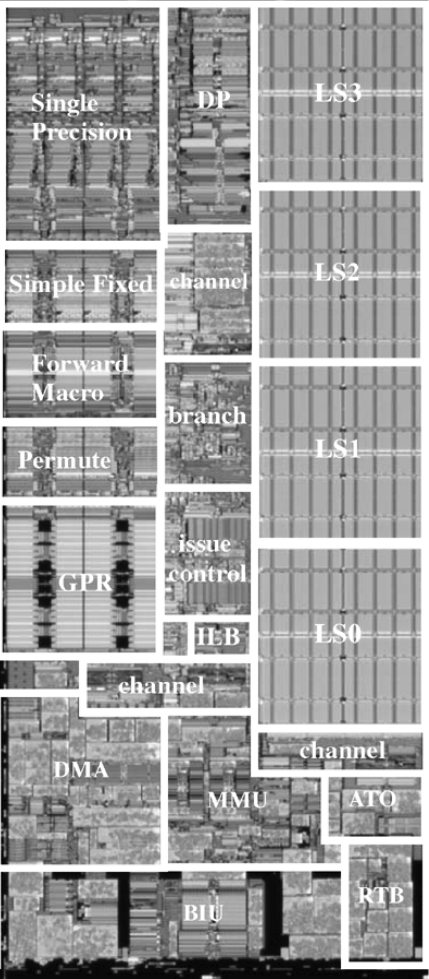
\includegraphics[scale=0.4]{./spe}
\caption{A photo of the SPE die}
\label{spe_die}
\end{figure}

\section{Experimental Results}

\subsection{Area Model Validation}

\subsection{Power Model Validation}

To validate our power model, we compare our model SPE's power consumption to the voltage/frequency shmoo published for an SPE in \cite{flachs2006microarchitecture}, both at 90nm. The published results we compare to are integer values only, which makes it difficult to judge the trend. We see that in the worst case, our model consumes 3x the power of the actual SPE, and 2x at a higher voltage ($V_dd = 1.3$). We can attribute this to several factors. First, our model uses a cache, which we know to draw more power than the local storage used in an SPE. Second, we know that STI designed several custom latches and latches \cite{pham2005design} to improve power efficiency and latency on the Cell, whereas McPAT has been validated against more commonly used hardware components.

\subsection{Energy Efficiency vs. Modern GPU}

We compare our Cell models to a modern GPU architecture. The AMD Radeon 7970 is an ideal candidate, as an example configuration is provided with Multi2Sim that has been validated against this architecture, and AMD has published results on its theoretical peak performance and power consumption. Released in 2012, the Radeon 7970 was built using a 28nm process, has a peak theoretical DP performance of over 1 TFLOPS, and a peak power draw of 250W \cite{radeon7970}. Therefore, it has a peak theoretical performance/power ratio of 4 GFLOPS/W. With a peak DP performance of 108.8 GFLOPS in the PowerXCell 8i, assuming we could scale this to 32 SPEs without running into further limitations, we would expect a peak theoretical DP performance of 435.2 GFLOPS on a 32 SPE Cell processor. For our 32 SPE Cell model, we quadruple all shared resources as well. We obtain a peak power consumption of 65 W, which using our theoretical peak performance gives a peak theoretical power efficiency of 6.7 GFLOPS/W. This result gives some hope that it may be possible for the Cell architecture to compete with GPGPUs, however, our performance modeling shows that the architecture cannot achieve anything near this peak theoretical performance.

\begin{table*}[t]
\centering
\begin{tabular}{| c | c | c | c | c | l |} \hline
\textbf{Category (McPAT)} & \textbf{Subcomponent} & \textbf{Actual (\%)} & \textbf{Actual ($mm^2$)} & \textbf{McPAT (\%)} & \textbf{McPAT ($mm^2$) }\\ \hline
\textbf{Instruction Fetch Unit}  & &  7.4\% & 1.09 & 10.0\% & 2.17 \\ \hline
  & Issue Control & 4.2\% & 0.61 & & \\ \hline
  & Branch Predictor & 3.2\% & 0.47  & & \\ \hline
\textbf{Load Store Unit}  & & 36.1\%  & 5.32 & 30.3\% & 6.58 \\ \hline
  & Local Storage & 29.2\% & 4.31 & & \\ \hline
  & DMA & 6.8\% & 1.01  & & \\ \hline  
\textbf{Memory Management Unit} &   6.8\% & 1.01 & 6.4\% & 1.39 \\ \hline
 &  MMU & 6.8\% & 1.01   & & \\ \hline  
\textbf{Execution Unit}  &  29.4\% & 4.33 & 27.6\% & 6.01  \\ \hline
 & Floating Point  & 13.8\% & 2.03      & & \\ \hline  
 &  Integer & 9.7\% & 1.44      & & \\ \hline  
 & Register File & 5.8\%  & 0.86      & & \\ \hline  
\textbf{Others} &   20.4\% & 3.01 & 25.8\% & 5.61  \\ \hline
 & Channels, etc. & 6.5\% & 0.96      & & \\ \hline  
 & Bus Interface Unit  & 9.4\%  & 1.39      & & \\ \hline  
 & Relational Translation Buffer & 4.5\% & 0.66      & & \\ \hline  
\textbf{Total}  & 100\%  & 14.75 & 100\% & 21.75   \\ \hline
\end{tabular}
\label{table:spe_area}
\end{table*}


\begin{figure}
\centering
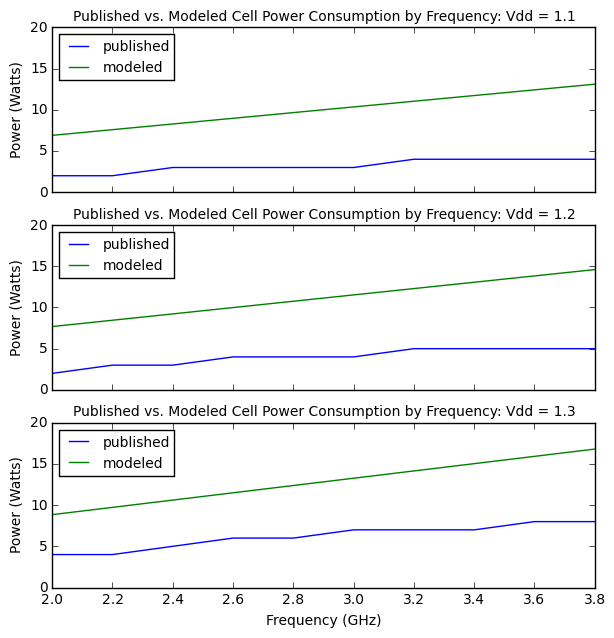
\includegraphics[scale=0.6]{./spe-voltage-freq}
\caption{Model vs. published power consumption for an SPE}
\label{spe-voltage-freq}
\end{figure}

\bibliographystyle{abbrv}
\bibliography{sigproc}  % sigproc.bib is the name of the Bibliography in this case
%
% The following two commands are all you need in the
% initial runs of your .tex file to
% produce the bibliography for the citations in your paper.
%\bibliographystyle{abbrv}
%\bibliography{sigproc}  % sigproc.bib is the name of the Bibliography in this case
% You must have a proper ".bib" file
%  and remember to run:
% latex bibtex latex latex
% to resolve all references

\end{document}
